On public cloud platforms, an Identity and Access Management (IAM) service is used to implement
authentication and authorization rules and policies for governing access to cloud resources.
IAM allows one to perform access control at a highly granular level with regard to who is allowed access and to what resource the access is allowed.
Whenn configured properly, IAM can provide an adequate level of protection for all resources and data through permissions and policies that are enforced on users and applications~\cite{AlmullaSameeraAbdulrahmanandYeun2010}.
IAM is first used to support the authentication of the identity of users or systems. For example, authentication between services involves often involves verifying an authentication token
passed from one endpoint to the other.  After authentication succeeds, IAM supports an
authorization process that determines the privileges afforded to a user or system and enforces
the security policies to ensure it.

\subsection{Basics}
In its instantiation on
Google Cloud Platform, there are three main components for implementing IAM: members, roles, and policies~\cite{Googlecloudiam}.  Members
provide the ``Identity'' (e.g. authentication) component while roles and policies provide the ``Access Management'' (e.g.
authorization) component.

\begin{figure}[h]
  \centering
  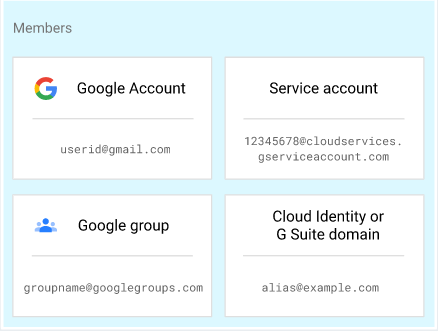
\includegraphics[width=\linewidth]{pic/mem}
  \caption {Types of Members in GCP}
  \label{fig:mem}
\end{figure}

\begin{figure}[h]
    \centering
    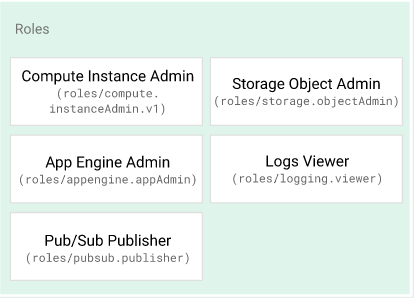
\includegraphics[width=\linewidth]{pic/role}
    \caption {GCP Predefined Role}
    \label{fig:role}
\end{figure}


\begin{itemize}
\item {\em Members} represent an authenticated identity.  As Figure~\ref{fig:mem} shows, such identities can be a Google user account
({\tt userid@gmail.com}), a service account created for applications ({\tt 1234...@....gserviceaccount.com}), a Google group ({\tt groupname@googlegroups.com}), or an identity domain ({\tt ...@example.com}). While the identities of the first three member types are email 
addresses, an identity domain is typically a domain name for an organization.

\item {\em Roles} are collections of permissions where each permission specifies access to and operations allowed on a particular resource.
Some examples of resources are projects, Compute Engine instances, and Cloud Storage buckets.  Due to the sheer number of 
resources in a cloud project, there are thousands of permissions that can be specified.  While one could assign individual
permissions to each member, doing so is quite cumbersome.  As a result, permissions are instead grouped and assigned to roles which are
then attached to members.  There are three types of roles supported in Google Cloud IAM \cite{googlecloudrole}: primitive, predefined and custom.
Primitive (also known as Basic) roles are coarse, project-level roles that are managed by GCP and include project ``Owner'', ``Editor'', and 
``Viewer'' roles.  Such roles existed prior to the current version of IAM in GCP that implemented finer-grained permissions and should not
be prevalently used to do the inability to reduce privileges in them appropriately.  Pre-defined roles are also maintained by GCP and
consist of collections of commonly grouped permissions for a specific service.  Pre-defined roles specify a permissions at a finer granularity 
than primitive roles and are made available to projects for convenience.  Figure ~\ref{fig:role} shows examples of several pre-defined roles that cover a variety of cloud platform resources and services.  There are instances when pre-defined roles do not exactly express an appropriate least privilege configuration for
a project.  In such cases, users can then create custom roles and specify the exact set of permissions
allowed.  This allows one to apply the PoLP at its finest granularity, but is the most complicated to set up, requiring the platform user to understand what individual permissions allow access to.
%%Custom roles provide user-specified list of permissions across services. Unfortunately, not all permissions can be linked to Custom roles such as Datastore related permissions.

\item {\em Policies} are collections of bindings that bind members to roles and thus give the members access to the resources specified in
each role.  Multiple members can be bound to a particular role~\cite{Googlecloudiam}. 
\end{itemize}

\begin{table}[t]
  \begin{center}
  \begin{tabular}{|p{4cm}|p{4cm}|}
  \hline
  Role & Permissions\\
  \hline
  \hline
  Storage Object Creator\par(roles/storage.objectCreator) &  resourcemanager.projects.get  \par resourcemanager.projects.list \par storage.objects.create \\ %% $\pm$ \\
  \hline
  Storage Object Viewer\par(roles/storage.objectViewer) & resourcemanager.projects.get\par resourcemanager.projects.list\par storage.objects.get\par storage.objects.list \\ %% $\pm$ \\
  \hline
  Storage Object Admin\par(roles/storage.objectAdmin) & resourcemanager.projects.get \par resourcemanager.projects.list\par storage.objects.*\\ %% $\pm$ \\
  \hline
  Storage HMAC Key Admin\par(roles/storage.hmacKeyAdmin) &storage.hmacKeys.*\\
  \hline
   Storage Admin\par(roles/storage.admin) &firebase.projects.get\par resourcemanager.projects.get\par resourcemanager.projects.list\par storage.buckets.*\par storage.objects.*\\
  \hline
  \end{tabular}
  \caption{IAM roles for Cloud Storage}
  \vspace{-0.20in}
  \label{table:sto-role}
  \end{center}
\end{table}

\begin{figure}[h]
\centering
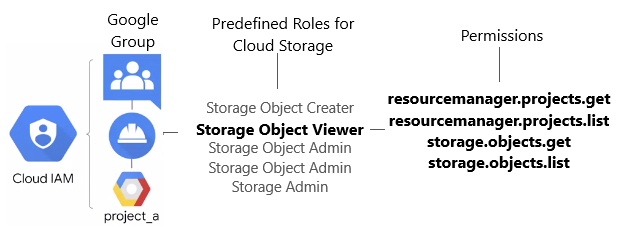
\includegraphics[width=\linewidth]{pic/sto-pre}
\caption {Policy - Predefined Role}
 \label{fig:sto-pre}
\end{figure}

\begin{figure}[h]
\centering
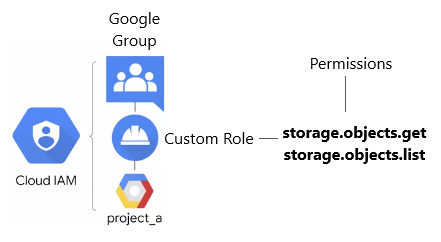
\includegraphics[width=\linewidth]{pic/sto-cus}
\caption {Policy - Custom Role}
 \label{fig:sto-cus}
\end{figure}

\subsection{An example applying least-privileges}
Consider a scenario in which two users need to list all of the objects in a storage bucket and view all of their contents.  To
begin with, we can define a member that is a Google group in which both users are added.  Then, for a policy, we can attach
a primitive role of project ``Viewer'' that will enable the users to view all parts of the project (not just its buckets).
The primitive role ``Viewer'', while having a limited set of permissions compared to the
primitive role ``Owner'', still has excessive permissions associated with it for the usage the two users require.
To address this, we might instead examine pre-defined roles defined for cloud storage as shown in Table~\ref{table:sto-role}
and attach a pre-defined role of ``Storage Admin'' ({\tt roles/storage.admin}) with its associated permissions.  Such a
setting would allow the operations ({\tt storage.objects.*}).  However, this also has excessive 
permissions. In looking at other pre-defined roles in the table and
their associated permissions with Cloud Storage, we notice that ``Storage Object Viewer'' has sufficient permissions
to list objects in a bucket ({\tt storage.objects.list}) and to retrieve an object's contents ({\tt storage.objects.get}).
Thus, binding ``Storage Object Viewer''
to the Google group would further reduce privileges as shown in Figure~\ref{fig:sto-pre}.
In looking at the ``Storage Object Viewer'' pre-defined role, however, we notice
that it provides two additional permissions that are not required by the two users.  To apply the PoLP at its finest granularity,
we can instead create a custom role and attach only the two permissions required.  As Figure~\ref{fig:sto-cus}, a custom role can then be defined
and a policy can be attached to the group in order to provide a least-privilege setting.
